\chapter{Introduction}
\label{cha:intro}

\epigraph{\textit{``If we want machines to think, we need to teach them to see.''}}{\textit{- Li Fei-Fei}}


As the most basic and influential part of human's sensory nervous system, vision plays a vital part in all kinds of recognition tasks. A glance at an image is sufficient for a human to point out and describe an immense amount of details about the visual scene. Traditionally, object recognition and description were performed manually. As time passed, the number of images in many systems grew to more substantial than terabyte size, and could no longer be maintained manually, which brought the idea of machine learning and computer vision also formed a part of artificial intelligence. 

The process of ``teaching machines to see'' has been widely discussed since the late 20$^{th}$ century and focused on modelling the 3D shape of objects. The latter focus emphasises the identification of objects, and this was achieved by adopting the AdaBoost \cite{adaboost} algorithm. Recently, since neural network-based algorithm AlexNet \cite{alexnet} won the object recognition ImageNet \cite{imagenet} competition in 2012, the field of computer vision began to make breakthroughs. At present, the top technology in the field of computer vision has been continuously approaching human performance. Besides, the learning mechanism, performance and security of neural networks are discussed in more depth.

\section{Computer Vision}

Computer vision (CV) refers to the ability of machines to perceive the environment, and it is the subject of researching machine vision capabilities, or the subject that enables machines to analyse the environment and the stimuli therein visually. Machine vision usually involves the evaluation of images or videos. The British Machine Vision Association (BMVA) defines machine vision as "the automatic extraction, analysis, and understanding of useful information from a single image or a series of images." \cite{bmva}

A real understanding of our environment is not achievable only by visual representation. More precisely, it is the process of transmitting visual cues to the primary visual cortex through the optic nerve, and then being analysed by the brain in a highly characterised form. Extracting explanations from this sensory information contains almost all of our natural evolution and subject experience, that is, how evolution survives us, and how we learn and understand the world in our lifetime.

In this respect, the visual process is only the process of transmitting images and interpreting them. However, from a computational point of view, the images are closer to thought or cognition and involve many functions of the brain. Therefore, due to the remarkable cross-domain characteristics, many people think that computer vision is a real understanding of the visual environment and its context, and will lead us to achieve reliable artificial intelligence.

\section{Motivation}
Image-text alignment is a fundamental research topic in the inter-field of computer vision and natural language processing. It will save the intense labour from annotating the artworks for online
digital artwork archives if we can automatically describe an artwork image or sub-image with its textual attributes. Furthermore, this topic can help to boost the multimodal question answering performance in the cultural heritage domain by providing fine-grained image-text correspondence information \cite{mqa}. Therefore, it is interesting to explore the methods that can figure out the artwork image or sub-image and text correspondence.

While a large number of papers discussed aligning image-text and coarse-grained modal information retrieval, the fragment level image-text alignment problem has not been as widely dealt within the multimodal question answering research domain. Coarse-grained modal information retrieval can retrieve information between image and text. However, it usually does not work well on artwork datasets which usually contain some fine-grained patterns and objects in one artwork image, therefore reduce the effectiveness of the retrieval model. In this section, we look at two simple examples of ancient Egyptian artworks and how textual description can be generated to match its image.

\begin{figure}[h!]
\centering
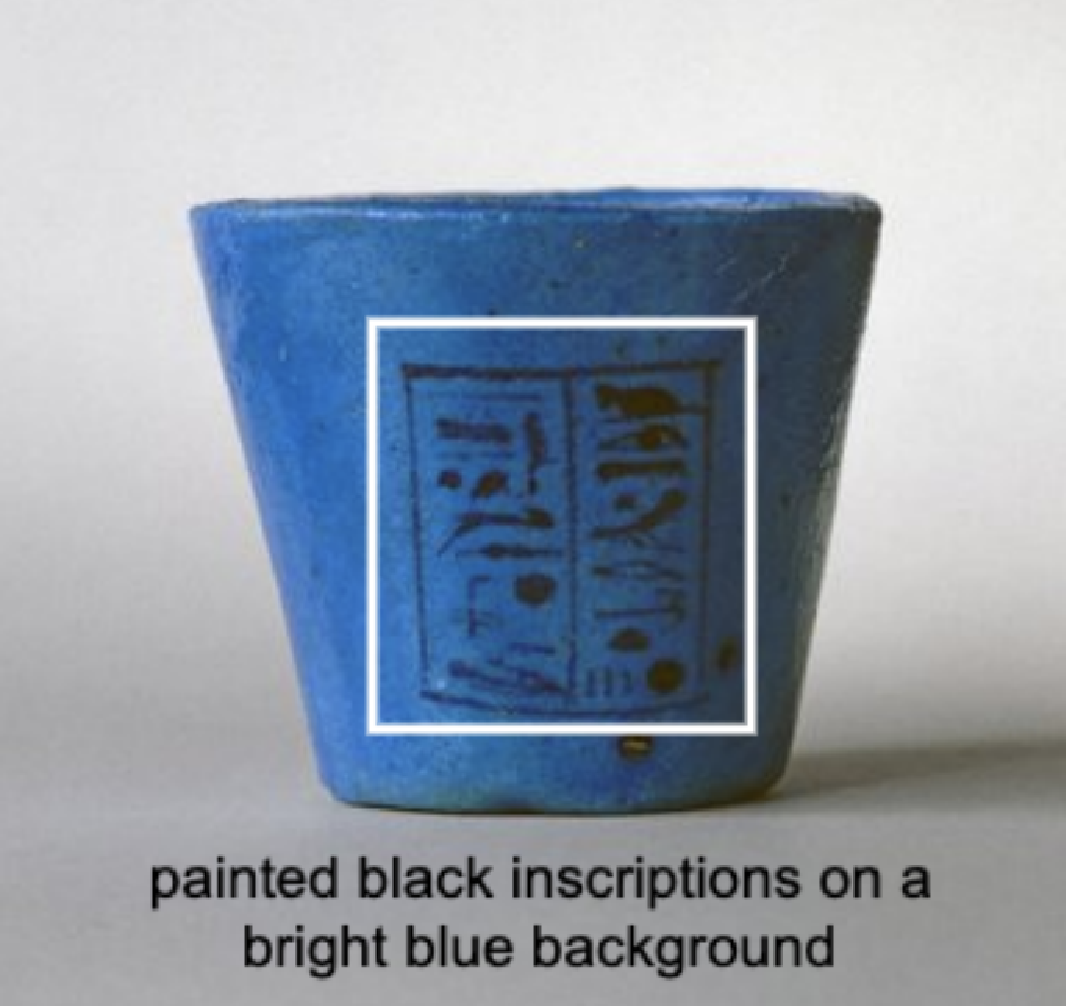
\includegraphics[width=0.35\textwidth]{artwork_fine1.pdf}
\caption{Ancient Egyptian artwork example (coarse-grained)}
\label{fig:artwork1}
\end{figure}

Figure \ref{fig:artwork1} shows a small blue container with black inked motifs on it. Using a coarse-grained multimodal retrieval model, we can generate the textual description ``\textit{painted black inscriptions on a bright blue background}'', which is sufficient enough for this artwork. However, in the real-world scenarios, there is much more likely for us to encounter an artwork showing in Figure \ref{fig:artwork2}. Our traditional coarse-grained multimodal retrieval model generates ``\textit{a red and a white pot}'' for this artwork but it is not detailed and did not cover sufficient information in the artwork image. Therefore, this motivated us to propose a fine-grained multimodal retrieval model which can focus on the fragment level image/sentence retrieval. The description on the image was generated by our fine-grained multimodal retrieval model, which has significantly more detailed information.

\begin{figure}[h!]
\centering
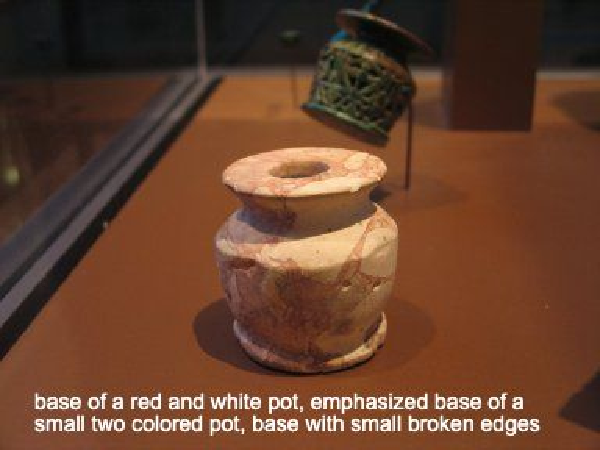
\includegraphics[width=0.45\textwidth]{artwork_fine2.pdf}
\caption{Ancient Egyptian artwork example (fine-grained)}
\label{fig:artwork2}
\end{figure}

\section{Dataset}

This thesis research is based on the dataset provided by \textit{The Rijksmuseum Challenge} \cite{MensinkICMIR2014}, which is posed from a museum-centric point of view offering a wide range of object types including paintings, photographs, ceramics, furniture, etc. The freely available dataset consists of 112,039 photographic reproductions of the artworks exhibited in the Rijksmuseum in Amsterdam, the Netherlands. 

The dataset has 112,039 high-quality artwork images recorded
in a controlled setting. Images are stored at 300 dpi and the
compressed \verb|jpeg| image file size ranges between 2-5 MB. There is a \verb|xml| file containing metadata corresponding to each image. However, in our research, instead of using the original captions in the \verb|xml| files, we extracted noun phrases from them and performed our alignment tasks between these noun phrases and images.

Here we focus on ancient Egyptian and Chinese artworks; we manually construct our datasets; they consist of 16,146 images from Egyptian domain and 6,847 images in Chinese. All metadata and textual
captions were originally recorded in Dutch, for the convenience of international collaboration, \textit{The Rijksmuseum Challenge} \cite{MensinkICMIR2014} also provided a cleaned and English version of all the textual captions. Figure \ref{fig:sampleEgyptian} and Figure \ref{fig:sampleChinese} show three examples of artworks from the Egyptian and Chinese collection with textual captions.

\begin{figure}[h!]
\centering
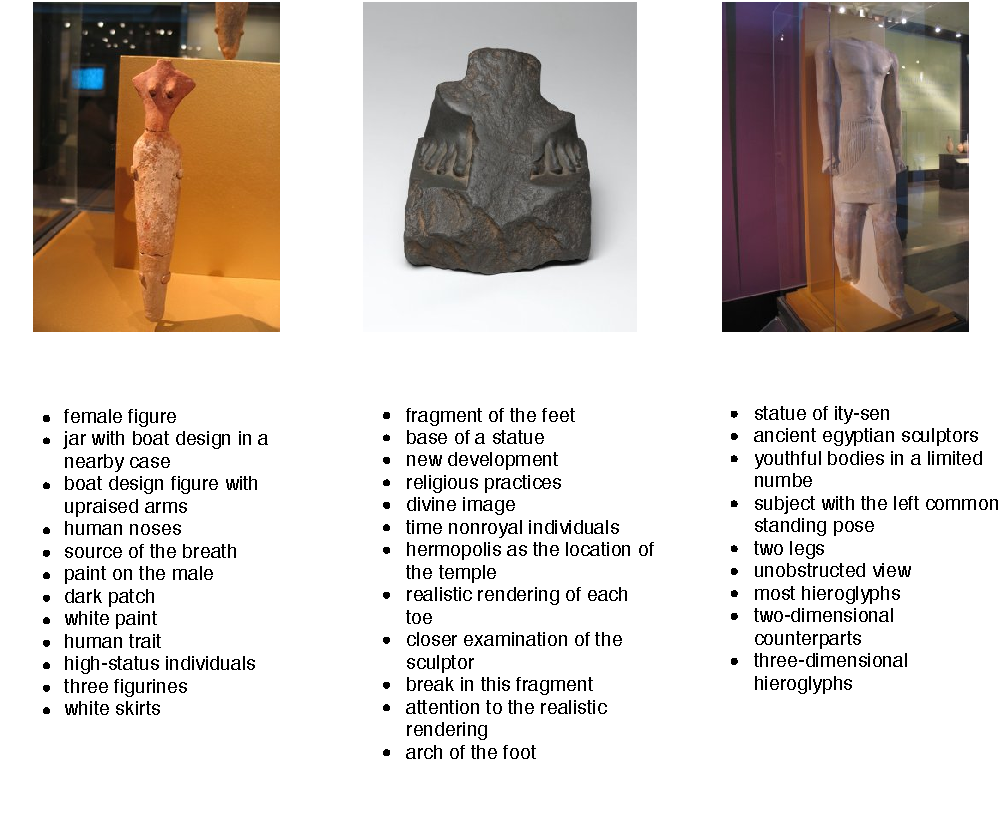
\includegraphics[width=0.6\textwidth]{egyptian.pdf}
\caption{Examples of artworks (image and textual data) of the Rijksmuseum dataset (Egyptian) \cite{MensinkICMIR2014}}
\label{fig:sampleEgyptian}
\end{figure}

\begin{figure}[h!]
\centering
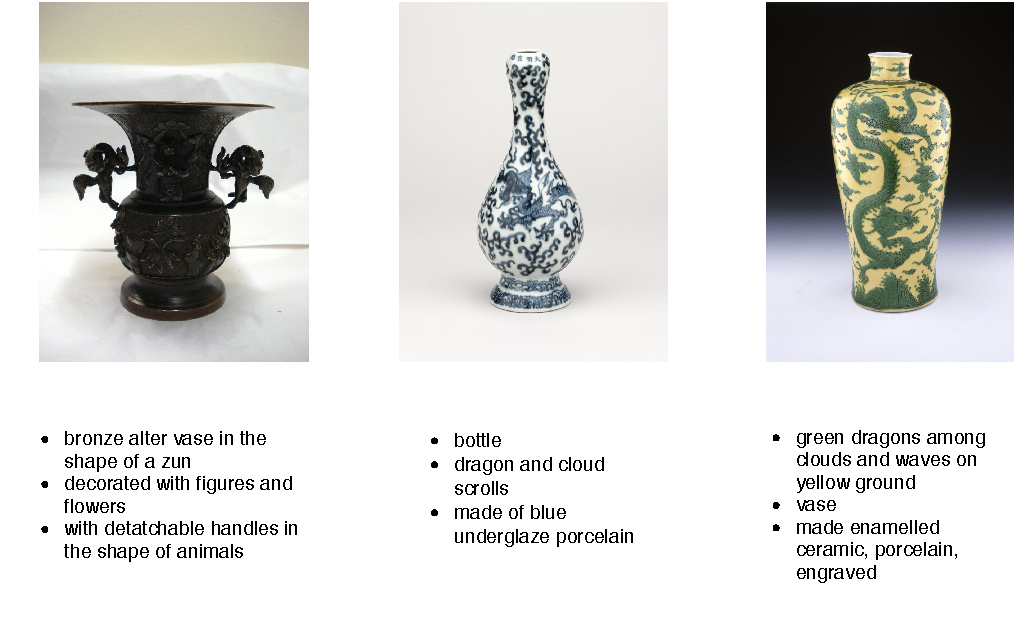
\includegraphics[width=0.6\textwidth]{chinese.pdf}
\caption{Examples of artworks (image and textual data) of the Rijksmuseum dataset (Chinese) \cite{MensinkICMIR2014}}
\label{fig:sampleChinese}
\end{figure}

\section{Research Questions}

In this thesis, we study fine-grained image-text alignment for artworks. Fine-grained image-text alignment refers to the fragment level cross-modal (between image and text) retrieval. The prior sections list the background and motivations, the specific research questions that we look at are:

\begin{itemize}
    \item Why mainstream coarse-grained image-text alignment techniques does not suit artwork domains well?
    \item Can we propose a practical approach that facilitates the textual attributes annotation of artwork images accurately and efficiently?
    \item Can we develop a fine-grained image-text alignment technique that can retrieve text from images and vice versa on fragment level?
\end{itemize}

\subsection{Cross Modal Retrieval Framework}

As mentioned above, our primary research task here is to achieve cross-modal retrieval (i.e. between image and text) for artworks. Figure \ref{fig:framework} illustrates a brief working framework for the tasks.

\begin{figure}[h!]
\centering
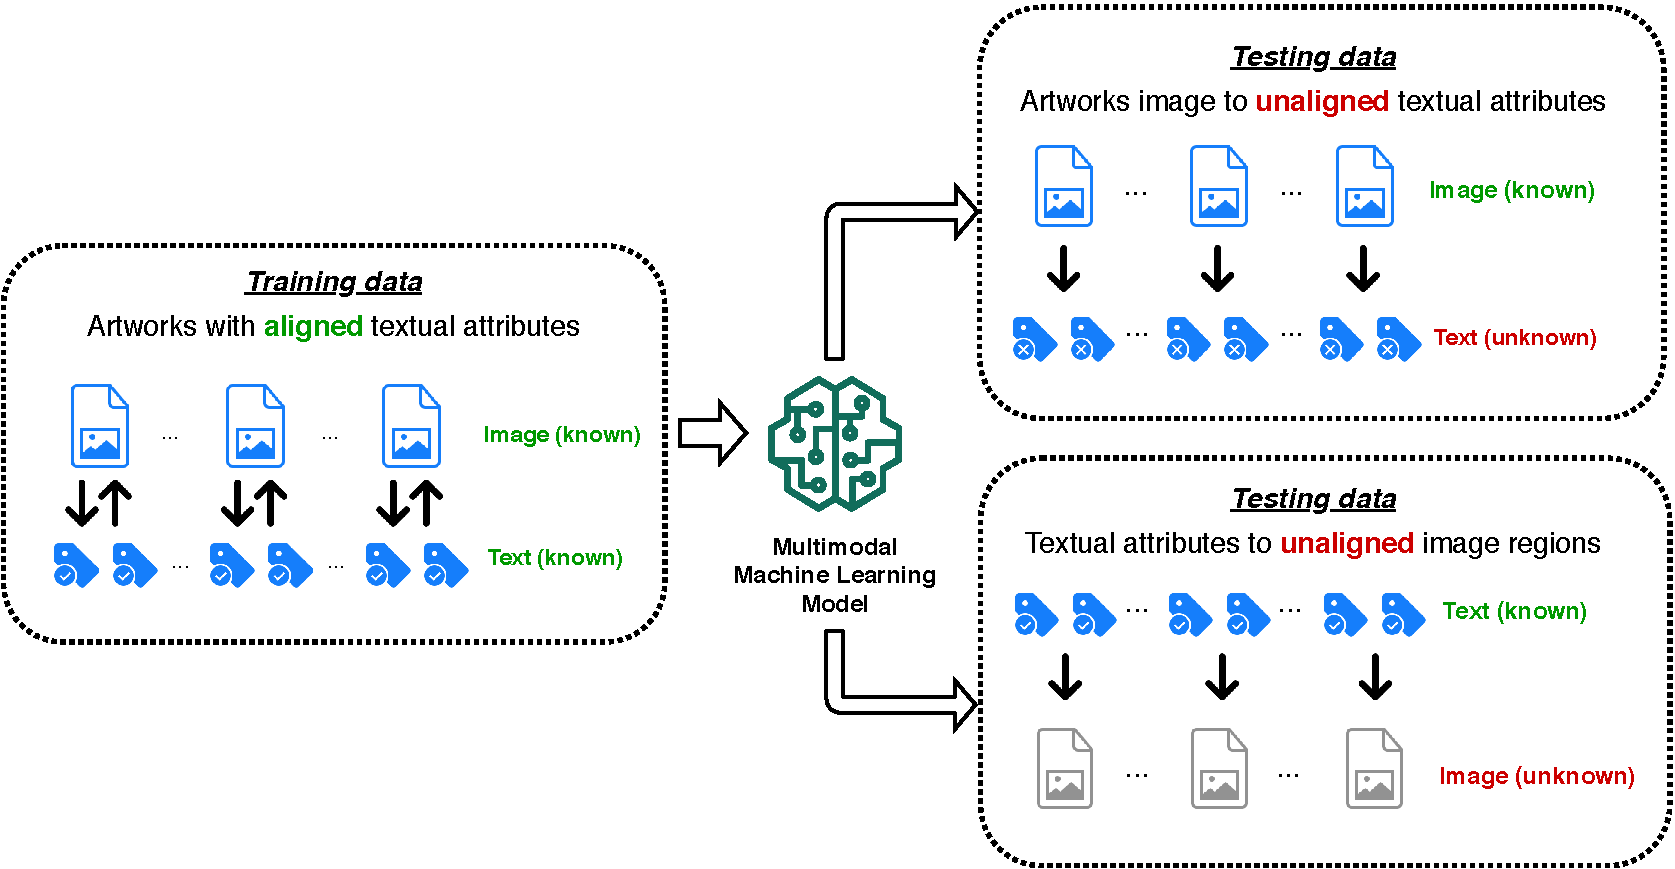
\includegraphics[width=\textwidth]{framework.pdf}
\caption{Cross Modal Retrieval Process}
\label{fig:framework}
\end{figure}

We train our multi-modal machine learning model on the known image features and corresponding textual attributes; this training process helps us learn the potential relationships between image and text. This trained model will be used to generate textual attributes from known image features and vice versa. We believe this may help with automating the artwork annotation process and significantly save labours on artworks classifications and searches.


\section{Contributions}
The main contributions made by this thesis are:

\begin{enumerate}
    \item We review work from several disciplines which may be of relevance to the present subject of inquiry and provide commentary on how the findings from these disciplines may be useful. (Section~\ref{cha:relatedworks})
    \item We adopted SCAN \cite{scan} as the coarse-grained cross-modal retrieval model, analysed its structure and applied it on our proposed Egyptian and Chinese artworks datasets to achieve the image-text alignment. With this baseline model, we are able to have a coarse-grained alignment between artworks image and textual attributes. This lays the foundation of our improved fine-grained model. (Section~\ref{cha:scan})
    \item By focusing on fragment level image features and textual attributes instead of feeding the whole images and sentences, we are able to perform cross-modal retrieval in a more fine-grained level. This allows the future multi-modal retrieval tasks on artworks to achieve more accurate and stable results. (Section~\ref{cha:Method})
\end{enumerate}


\section{Structure of Thesis}

This thesis is structured into the following chapters:

\begin{itemize}
    
    \item \textit{Section~\ref{cha:intro} Introduction}\newline
    We provide the reader with a relevant background to understand this thesis.

    \item \textit{Section~\ref{cha:relatedworks} Related Works}\newline
    We introduce relevant research in image recognition, deep learning, object detection, natural language processing and image-text alignment. In particular, we detail seminal research and review the overall state of the current research. We also review the difference in the works pertaining to the traditional visual-semantic alignment technique versus the more recent cross attention image-text alignment framework.
    
    \item \textit{Section~\ref{cha:scan} Coarse-grained Cross-Modal Retrieval}\newline
    We introduce our coarse-grained cross-modal retrieval modal - SCAN, discuss how its components interact with each other and explain how SCAN uses cross attention to improve image-text alignment. We also show the preliminary result running SCAN on our ancient Egyptian and Chinese artwork datasets.
    
    \item \textit{Section~\ref{cha:Method} Fine-grained Cross-Modal Retrieval}\newline
    We proposed our improved fine-grained cross-modal retrieval model, which now focus more on the fragment level image-text alignment. We then perform several experiments on evaluating the effectiveness of our image generation from text and vice versa by the recall. We also point out the direction of possible future improvements by discussing several recent related publications.
    
    \item \textit{Section~\ref{cha:conclusion} Conclusion}\newline
    We conclude the work and add some final reflections and remarks.
\end{itemize}
%%% Local Variables: 
%%% mode: latex
%%% TeX-master: "thesis"
%%% End: 
